%
%
%
\chapter{The Static Conductivity in the Spin Fermion Model including Umklapp Scattering}
\label{ch:calculation}
%
%
%
The static electrical conductivity $\sigma_{\mt{dc}}$ is computed in this chapter, using the memory-matrix-formalsim.
The underlying model is the spin-fermion-model (see chapter \ref{ch:spin fermion model}), including umklapp scattering as a translation symmetry breaking pertubation.
In this chapter, our attention is focused on the physical analysis of the obtained expression for the conductivity.
An explicite computation is demonstrated in appendix \ref{app:calculation}
%
%
%\section{Static Conductivity's Derivation}
%\label{sec:deviation conductivity}
%
%
Two physical objects, fermions near the Fermi surface and spin fluctuations, are considered in the spin-fermion-model, introduced in the previous chapter.
Spin fluctuations are generated at the vicinity of an antiferromagnetic quantum critical point due to particle-holes-excitations.
Fermions, located at the point $\vb{k}$ and $\vb{k}+\vb{Q}$ on the Fermi suface, are connected to each other because of these fluctuations.
In the previous chapter, it is shown that the model Hamiltonian of the spin-fermion-model is conserved the momentum.
The static electrical conductivity is thus infinite as it is poven in chapter \ref{ch:infinite conductivity}.
Considering umklapp scattering, the translation symmetry is broken and the momentum is unconserved.
As a conseuqence the static conductivity becomes finite, which is computed in the following.

In chapter \ref{ch:memory matrix formalism} over the memory-matrix-formalism, the following formula is derivated for the static electrical conductivity, considering the spin-fermion-model and umklapp scattering.
%
\begin{align}
	\sigma_{\mt{dc}} = -\lim\limits_{z \to 0} \frac{z \cdot |\chi_{\mt{JP}}(\omega = 0)|^{2}}{\mathcal{G}_{\dot{\mt{P}}\dot{\mt{P}}}(\vb{k}, z)}
	\label{eq:static conductivity formula}
\end{align}
%
Here, $z$ is a complex frequency and $\chi_{\mt{JP}}(\omega = 0)$ is the static susceptibility between current and momentum.
In the denominator the Green function is given by
%
\begin{align}
	\mathcal{G}_{\dot{\mt{P}}\dot{\mt{P}}}(\vb{k}, z) = \int\limits_{0}^{\infty} \dd{t} e^{izt} \expval{\comm{\dot{\mt{P}}(t)}{\dot{\mt{P}}(0)}_{-}}_{0},
	\label{eq:Green function}
\end{align}
%
where the usual quantum mechanical commutator is used, indicated with the minus sign at the squared brackets.
The expectation value is generated with respect to the unpertubative Hamiltonian H, illustrated with the index 0.
Here, the interaction between fermions and spin fluctuations is included.
The time derivative of momentum is given by equation \eqref{eq:time derivative momentum finite}.

The Green function $\mathcal{G}_{\dot{\mt{P}}\dot{\mt{P}}}(\vb{k}, z)$ and the static susceptibiliy $\chi_{\mt{JP}}(\omega = 0)$ are investigated, due to their possible temperature dependence.
The latter is expected to be temperature independent.
\todo{Why? -> P and J are explicitely time independent}
This is computed in detail in the appendix \ref{app:calculation}, using the diagrammatic pertubation technique.
The considered diagrams are the electron-pair bubble for each species of fermions, depicted in figure \ref{fig:bubble electrons}.
Therefore, the obtained expression of the susceptibility is given by
%
\begin{align}
	\chi_{\mt{PJ}}(\omega = 0) = \frac{\sqrt{m_{1} m_{2}}}{\pi} T \cdot \ln(e^{\flatfrac{\mu}{T}} + 1),
	\label{eq:static susceptibility computed}
\end{align}
%
where the chemical potential is denoted as $\mu$.
The logarithm is approximated in the limit of small temperatures ($\mu \gg T$) to $\ln(e^{\flatfrac{\mu}{T}} + 1) \rightarrow \flatfrac{\mu}{T}$.
Inserting this expression, the temperature is canceled and the static susceptibility is given by constant parameters, $\chi_{\mt{PJ}}(\omega = 0) = \flatfrac{\mu\sqrt{m_{1} m_{2}}}{\pi}$.
The chemical potential is assumed as temperature independent in the observed regime.

%
\begin{figure}
	\centering
	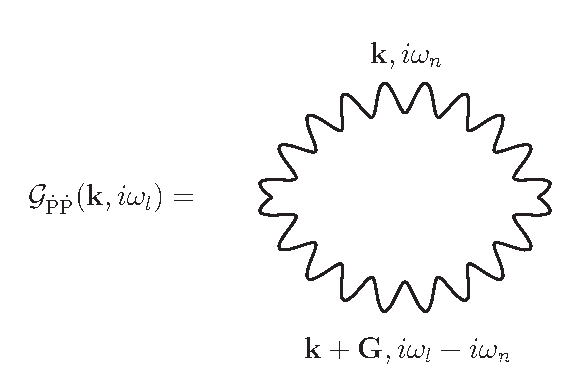
\includegraphics[width=0.4\textwidth]{spin_wave_bubble.eps}
	\caption{caption}
	\label{fig:spin wave bubble}
\end{figure}
%
The only temperature dependence of the static electrical conductivity is hence emerged by the Green function $\mathcal{G}_{\dot{\mt{P}}\dot{\mt{P}}}(\vb{k}, z)$.
Only the free bubble diagram is considered computing the Green function with diagrammatic pertubation theory, which is depicted in figur \ref{fig:spin wave bubble}.
Higher order terms in the diagrammatic treatment are corrections of the bubble diagram and since spin fluctuations are the observing objects only bubble diagrams occur.
Therefore the conductivity or resistance is only determined by spin fluctuations.
Resistance is a consequence of fermionic coupling to other degrees of freedom, obtained as finite fermionic lifetime.
The resistance is thus proportional to the imaginary part of the retarded Green function $\mathcal{G}_{\dot{\mt{P}}\dot{\mt{P}}}^{\mt{ret}}(\vb{k}, z)$.
Appendix \ref{app:calculation} is shown the detailed computation of the expression of the retarded Green function.
%
\begin{align}
	\Im{\mathcal{G}_{\dot{\mt{P}}\dot{\mt{P}}}^{\mt{ret}}(\vb{k}, z)} &= 
		-\frac{4 \gamma^{2} \beta \omega}{\pi}
		\sum\limits_{\vb{Q}_{1}, \vb{Q}_{2}}
		\sum\limits_{\vb{G}}
		\vert \mt{J}_{\vb{G}} \vert^{2}
		\int\limits_{0}^{\infty} \dd{\epsilon}
		\frac{\epsilon^{2} e^{\beta \epsilon}}{(e^{\beta \epsilon} - 1)^{2}}
		\notag \\
		&\times
		\int_{\vb{k}} G_{j}^{2} \cdot
		\frac{1}{(\vb{k}+\vb{G}-\vb{Q}_{1})^{4} + \gamma^{2} \epsilon^{2}} \cdot
		\frac{1}{(\vb{k} + \vb{Q}_{2})^{4} + \gamma^{2} \epsilon^{2}}
\end{align}
%
Here the term under the momentum integral is given by the imaginary part of the damped spin density propagator, denoted in \eqref{eq:damped spin propagator real axis}.
The integral itself is extended over the first Brillouin zone.
The periodicity of the spin susceptibility and pertubation is considered by the sums over $\vb{Q}_{i}$ ($i=1,2$) and $\vb{G}$, respectivily.
In both cases these are reciprocal lattice vectors.
Spatial direction of the momentum is represented by the index $j$ and $\beta^{-1} = T$.

The obtained integrals is now investigated with respect to different cases since their are not exactly solvable.
A detailed discussion of the single cases and an approximated computation of the integral is demonstrated in the following.

%
%
%\section{Analysis of the static conductivity}
%\label{sec:analysis conductivity}
%
%
Convergence of the intergal is surely given, if one of the momentum terms, $\vb{k}+\vb{G}-\vb{Q}_{1}$ or $\vb{k} + \vb{Q}_{2}$, is large according to amount.
Since both terms are of the power of four, the integral is a fast decreasing function in the large momentum limit.
Nevertheless, divergences of the integral are reached, if these terms are zero and this happens in many cases.
One of the most divergent cases is assumed in the following approach.
The vector $\vb{k}$ is limited on the first Brillouin zone and the reciprocal lattice vectors are set to $\vb{G} = \vb{Q}_{1}$ and $\vb{Q}_{2} = 0$.
The choice of the reciprocal lattice vectors is arbitrary and it is therefore possible that the $j$-component of $\vb{G}$ is large.
This divergence is canceled by the coupling parameter $\mt{J}_{\vb{G}}$ assumed as fast decreasing for large $|\vb{G}|$.

The remaining momentum integral is now exactly integrable.
First of all, the momentum and frequency variables are transformed into dimensionles variables, using the transformation rules $\vb{k} = \vb{y} \cdot \sqrt{\gamma T}$ and $\epsilon = x \cdot T$, respectivily.
The new variable $\vb{y}$ is further transformed into plane polar coordinates.
The upper limit of the radius $|\vb{y}|$ is set to infinity, since the integrand is decreasing fast to zero for $|\vb{y}| \to \infty$.
As a consequence the angular integral is easily evaluated, yielding the factor $2\pi$.
The remaining integral is given by the following expression.
%
\begin{align}
	\Im{\mathcal{G}_{\dot{\mt{P}}\dot{\mt{P}}}^{\mt{ret}}(\vb{k}, z)} = 
		 -\frac{2 \cdot G_{j}^{2} \cdot \vert \mt{J}_{\vb{K}} \vert^{2}}{\gamma \cdot \pi^{2}} \cdot \frac{\omega}{T}
		\int\limits_{0}^{\infty} \dd{x}
		\frac{x^{2} e^{x}}{(e^{x} - 1)^{2}}
		\int\limits_{0}^{\infty} \dd{y}
		\frac{y}{\big(y^{4} + x^{2}\big)^{2}}
\end{align}
%
The $y$-integral is substituted one last time, using the transformation rule $y^{2} = z \cdot x$.
The obtained integral is evaluated to $\flatfrac{\pi}{4}$, using the integral formula \eqref{eq:integral1}.
Both limits, $x \to 0$ and $x \to \infty$, of the intergal over $x$ are investigated.
In the case of large $x$, the integral is decreasing fast to zero due to the ratio of the exponential functions.
The upper limit is thus set to one and the integrand is expanded for small values of $x$.
In first order the integrand is approximated to $\flatfrac{1}{x^{3}}$.
This is a highly divergent function in the limit $x \to 0$ and as a consequence the static conductivity is divergent as well.

The result of a divergent conductivity is clearly incorrect in a system with broken translation symmetry.
In chapter \ref{ch:infinite conductivity}, it is shown that translation symmetry and the consequent conserved momentum is caused an infinite conductivity in the static limit.
As showing in chapter \ref{ch:spin fermion model}, momentum is conserved in the unpertubated spin-fermion-model (equation \eqref{eq:time derivative momentum}) and it is thus a system with unbroken translation symmetry.
Momentum is unconserved (equation \eqref{eq:time derivative momentum finite}), introducing umklapp scattering as an observing pertubation.
A finite conductivity is now expected, instead of a divergent one.

Our supposed correct choice of the control parameter $r$ is the origin of this discrepancy.
The paramter $r$ is assumed to be zero, since its proportional to $\xi^{-2}$ and the correlation length $\xi$ is divergent at the quantum critial point.
This assumption is incorrect in the sence that the system is not directly at the quantum cirtical point, but rather in the vicinity of him.
The system is supposed to be in the quantum critical phase, depicted in the phase diagram \ref{fig:phase diagram}, at a point with tuning parameter $\mt{g} = \mt{g}_{\mt{c}}$ and temperature $ T > 0$.
While the temperature is decreased to get closer to the quantum critical point, the tuning parameter is fixed.
Considering the finite value of the control parameter $r$, the imaginary part of the retareded Green function is given by
%
\begin{align}
	\Im{\mathcal{G}_{\dot{\mt{P}}\dot{\mt{P}}}^{\mt{ret}}(\vb{k}, z)} &= 
		-\frac{4 \gamma^{2} \beta \omega}{\pi}
		\sum\limits_{\vb{Q}_{1}, \vb{Q}_{2}}
		\sum\limits_{\vb{G}}
		\vert \mt{J}_{\vb{G}} \vert^{2}
		\int\limits_{0}^{\infty} \dd{\epsilon}
		\frac{\epsilon^{2} e^{\beta \epsilon}}{(e^{\beta \epsilon} - 1)^{2}}
		\notag \\
		&\times
		\int_{\vb{k}} G_{j}^{2} \cdot
		\frac{1}{((\vb{k}+\vb{G}-\vb{Q}_{1})^{2} + r)^{2} + \gamma^{2} \epsilon^{2}} \cdot
		\frac{1}{((\vb{k} + \vb{Q}_{2})^{2} + r)^{2} + \gamma^{2} \epsilon^{2}}
\end{align}
%
The approach is nearly the same for solving the integrals as previously.
Firstly, the convergence of large values of momenta is not changed, because of considering $r$.
One of the most divergent cases is stil $\vb{G} = \vb{Q}_{1}$ and $\vb{Q}_{2} = 0$.
Furthermore, the divergence, generated by large values of $G_{j}$, is still canceled since the coupling parameter $\mt{J}_{\vb{G}}$ is decreased fast in the limit $|\vb{G}| \to \infty$.
The remaining momentum integral is of the same structure as above and exactly solvable.
Therefore, the momentum integral is firstly transformed into plane polar coordinates, $\vb{k} = (k\cos\phi, k\sin\phi)$.
The upper limit of $k$ is again set to infinity, since the integrand is fast decreasing to zero for $k \to \infty$ and the contributions are neglectable.
%
\begin{align}
	\Im{\mathcal{G}_{\dot{\mt{P}}\dot{\mt{P}}}^{\mt{ret}}(\vb{k}, z)} &= 
		-\frac{\vert \mt{J}_{\vb{G}} \vert^{2} \cdot G_{j}^{2}}{\gamma \pi^{2}} \cdot 
		\frac{\omega}{T}
		\int\limits_{0}^{\infty} \dd{\epsilon}
		\frac{\epsilon^{2} e^{\beta \epsilon}}{(e^{\beta \epsilon} - 1)^{2}}
		\int\limits_{0}^{\infty} \dd{k}
		\frac{k}{((r + k^{2})^{2} + \gamma^{2} \epsilon^{2})^{2}}
	\label{eq:starting expression}
\end{align}
%
where the angular integral is performed.
The obtained momentum integral is substituted using $z = \flatfrac{(r + k^{2})}{\gamma\epsilon}$.
In comparison to the case above, the lower limit is changed to $\flatfrac{r}{\gamma \epsilon}$.
Both cases are equivalent in the limit $r \to 0$.
The finite lower boundary guarantees the convergence of the remaining integral over $\epsilon$.
The integral over $z$ is performed, utilizing the integral formula \eqref{integral1} again.
Dimensionless variables are introduced, using $x = \beta \epsilon$.
The obtained expression is given by
%
\begin{align}
	\Im{\mathcal{G}_{\dot{\mt{P}}\dot{\mt{P}}}^{\mt{ret}}(\vb{k}, z)} &= 
		-\frac{\vert \mt{J}_{\vb{G}} \vert^{2} \cdot G_{j}^{2}}{4 \gamma \pi^{2}} \cdot 
		\frac{\omega}{T}
		\notag \\
		\times &\int\limits_{0}^{\infty} \dd{x}
		\frac{1}{x} \frac{e^{x}}{(e^{x} - 1)^{2}} \cdot
		\bigg[\pi - \frac{2 \flatfrac{\tilde{r}}{x}}{(\flatfrac{\tilde{r}}{x})^2 + 1} - 2 \arctan(\flatfrac{\tilde{r}}{x})\bigg],
\end{align}
%
where the abbreviation $\tilde{r} = \flatfrac{r}{\gamma T}$ is introduced.
The integral over $x$ is not analytical exactly solvable.
However, the integral is finite in both limits, $x \to 0$ and $x \to \infty$.
The latter is surely statisfied.
The ratio of exponential functions is fast decreasing to zero and no other term is divergent.
In the limit $x \to 0$, the integrand is limited by $\flatfrac{4}{3r^{3}}$, which is only divergent for $r \to 0$.
The behaviour of the integrand is depicted on left hand side in figure \ref{fig:behaviour integrand}, setting $\tilde{r} = 2$.
%
\begin{figure}[t]
	\centering
	\subfigure[]{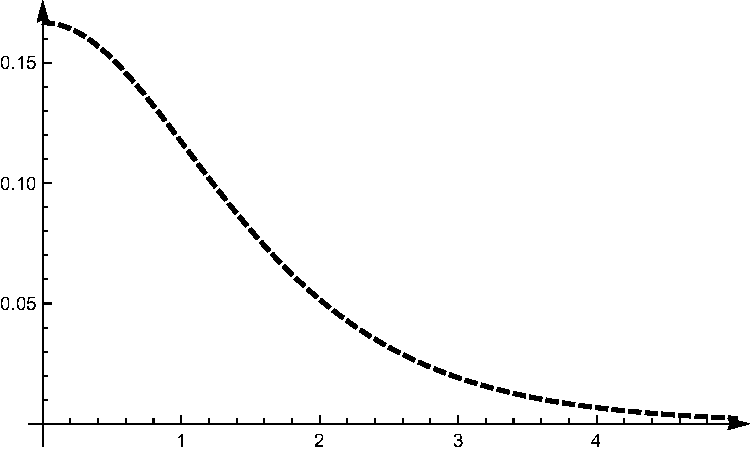
\includegraphics[width=0.49\textwidth]{behaviour_integrand.pdf}}
	\subfigure[]{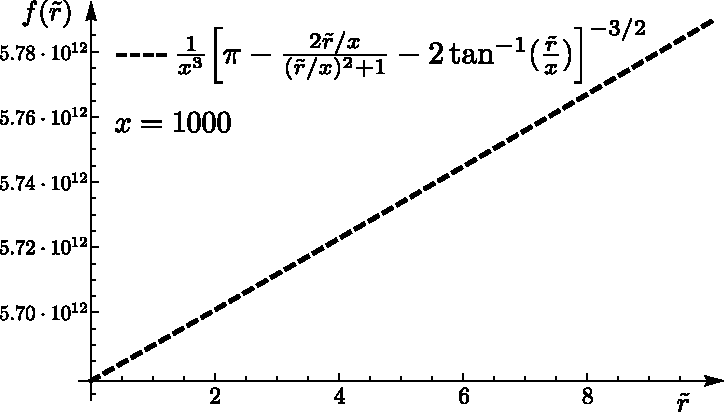
\includegraphics[width=0.49\textwidth]{dependence_integrand.pdf}}
	\caption{caption}
	\label{fig:behaviour integrand}
\end{figure}
\todo{rechtes Bild korrigieren}
%
A solution of the integral is evaluated determining the behaviour of the expression in squared brackets.
For large values of $x$, a linear $r$-dependence is given by the power of $-\flatfrac{2}{3}$.
This is depicted in the right hand side of figure \ref{fig:behaviour integrand}, where $x$ is set to 100.
An approximated expression is generated for the interand using the method of power counting.
The initial point of this approach is the momentum integral in euqtion \eqref{eq:starting expression}.
Numerator and differatial yield in total the power of two, while the denominator generates the power of eight.
Combining both, the integrand is a function proportional to $k^{-6}$.
The further approach is now to investigate singularities of the integrand.
The limit $r \to 0$ or $\epsilon \to 0$ is seperately generated singularities in the function.
Both are considered with the power of three, since the power of them is half in comparison to the power of $k$ in equation \eqref{eq:starting expression}.
The integrand is therefore approximated by the following expression.
%
\begin{align}
	\Im{\mathcal{G}_{\dot{\mt{P}}\dot{\mt{P}}}^{\mt{ret}}(\vb{k}, z)} &\approx 
		-\frac{2 \vert \mt{J}_{\vb{G}} \vert^{2} \cdot G_{j}^{2}}{\gamma \pi^{2}} \cdot 
		\frac{\omega}{T}
		\int\limits_{0}^{\infty} \dd{x}
		\frac{x^{2} e^{x}}{(e^{x} - 1)^{2}}
		\frac{1}{(\tilde{r}^{2} + x^{2})^{\flatfrac{3}{2}}}
\end{align}
%
In figure \ref{fig:integrand exact vs approx}, the approximated expression is confronted with the exact one.
The behaviour of both are nearly identical and the estimation is inspected as valid.
The integrand is still decreasing fast to zero for $x \to \infty$, while the upper limit is set to some arbitrary cut-off $\Lambda$.
%
\begin{figure}[t]
	\centering
	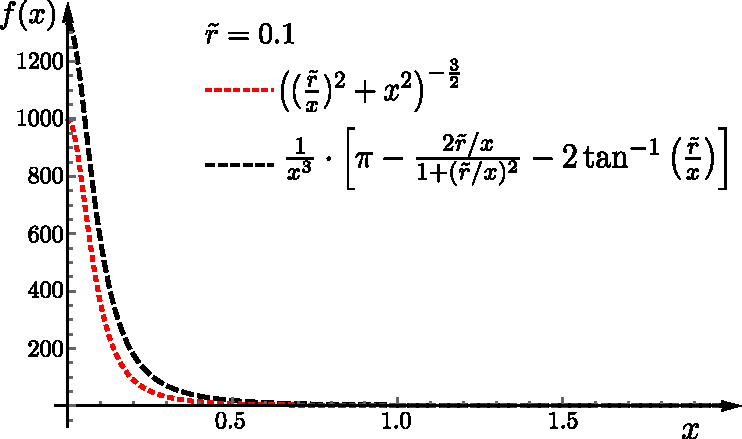
\includegraphics[width=0.6\textwidth]{original_vs_powercounting.pdf}
	\caption{caption}
	\label{fig:integrand exact vs approx}
\end{figure}
%
The ratio of the exponential functions are then expanded for small values of $x$ up to the first non-vanishing order.
The remained integral is exactly solvable and expanding the solution for small $\flatfrac{\tilde{r}}{\Lambda}$ the solution of the integral is given by
%
\begin{align}
	\Im{\mathcal{G}_{\dot{\mt{P}}\dot{\mt{P}}}^{\mt{ret}}(\vb{k}, z)} &\approx 
		-\frac{2 \gamma \vert \mt{J}_{\vb{G}} \vert^{2} \cdot G_{j}^{2}}{\pi^{2} \Lambda} \cdot \frac{\omega T}{r^{2}}
\end{align}
%
Inserting this expression and the approximated static susceptibility of \eqref{eq:static susceptibility computed} into equation \eqref{eq:static conductivity formula}, the static electrical conductivity is given by
%
\begin{align}
	\sigma_{\mt{dc}}(T) = \frac{\mu\: m_{1}\: m_{2}\: \Lambda}{2\: \gamma\: \vert \mt{J}_{\vb{G}} \vert^{2}\: G_{j}^{2}} \cdot \frac{r^{2}}{T}
\end{align}
%
Beside the temperature itself, the only temperature dependent parameter is the control parameter $r$, which is proportional to the squard inverse correlation length, $r = \xi^{-2}$.
The correlation length is originated due to the fact that the system possesses a quantum phase transition and is temperature dependent is given by $\xi = T^{-1/z}$, as shown in chapter \ref{ch:spin fermion model}.
$z$ is a critical exponent and it is chosen in dependence of the distance to the qantum critical point.
The corresponding temperature depencence of the control parameter is therefore provided to $r = T^{2/z}$.
The resistance is determined by the inverse of the conductivity.
Considering only the temperature dependent parameter, the static resistance is given by
%
\begin{align}
	\rho_{\mt{dc}}(T) \sim T^{1-\flatfrac{4}{z}}
	\label{eq:solution resistance}
\end{align}
%
Two possible choices are mentioned for the ciritcal exponent $z$ in chapter \ref{ch:spin fermion model}.
In the vicinity of the quantum critical point at higher temperatures, $z$ is chosen to be one.
The $T$-dependence of the resistance is then given by $T^{-3}$.
In the limit $T \to 0$, this is highly divergent.
$z$ is chosen to be two for lower temperatures.
Nevertheless, the $T$-dependence is evaluated to $T^{-1}$, which is still divergent in the limit $T \to 0$.

Our physial expectation is not confirmed with this divergent behaviour of the resistance.
Experiments of the investigated metals \cite{Loehneysen} are shown a linear temperature dependence of the resistance, $\rho(T) = \rho_{0} + A\: T$.
The behaviour of the resistance is described incorrect with our obtained solution \eqref{eq:solution resistance}.
A possible origin of this disgrepancy between experiemnt and theory is maybe the diagrammatic pertubation theory.
In equation \eqref{eq:Green function}, the time evolution operator is expanded up to the first non-vanishing order.
This yields the free bubble diagram, while correction to the bubble are considered  expanding the time evolutaion operator up to the next order.







%In Landau's Fermi liquid theory the resistance of a metal is given by $\rho(T) = \rho_{0} + A\: T^{2}$, where the residual resistance due to impurity scattering is represented by $\rho_{0}$.
%The $T^2$-dependence is originated by electron-electron scattering and umklapp-scattering \cite{Bader, Pal}


%In \cite{Loehneyesen} metals are investigated where a non-Fermi liquid behaviour 
%The consideration of umklapp scattering 

%Both results do not describe the physical results, presented in \cite{Loehneysen}.
%Here, 

%coincide 


















